\documentclass{beamer}
% francification de LaTeX
\usepackage[utf8]{inputenc}
\usepackage[french]{babel}
% imagination
\usepackage{tikz}
% options de beamer
\usetheme{Boadilla}
\title{Projet \textit{Labyrinthe}}
\subtitle{Algorithmes et Structures de Donnée}
\author{Juan-Carlos Barros et Daniel Kessler}
% des compteurs pour l'importation d'images
\usepackage{forloop}
\newcounter{onlynumber}
\newcounter{pngnumber}
% et c'est parti
\begin{document}

\begin{frame}
  \titlepage
\end{frame}

\begin{frame}
%  \frametitle{}
  % Formation \textit{GymInf},
  Cours d'\textit{\textcolor<1>{blue}{Algorithmes}}
  et \textit{\textcolor<1>{green}{Structures de donnée}}
  \par\bigskip
  \onslide<2->{Projet \textit{Labyrinthe}}\par
  \begin{minipage}{.5\linewidth}
  \begin{itemize}
  \item<2->\textcolor{blue}{Algorithme}\par\onslide<3->{A*}
  \item<2->\textcolor{green}{Structure de Donnée}\par\onslide<4>{Priority Queue}
  \end{itemize}
  \end{minipage}
  \begin{minipage}{.3\linewidth}
  \onslide<2->{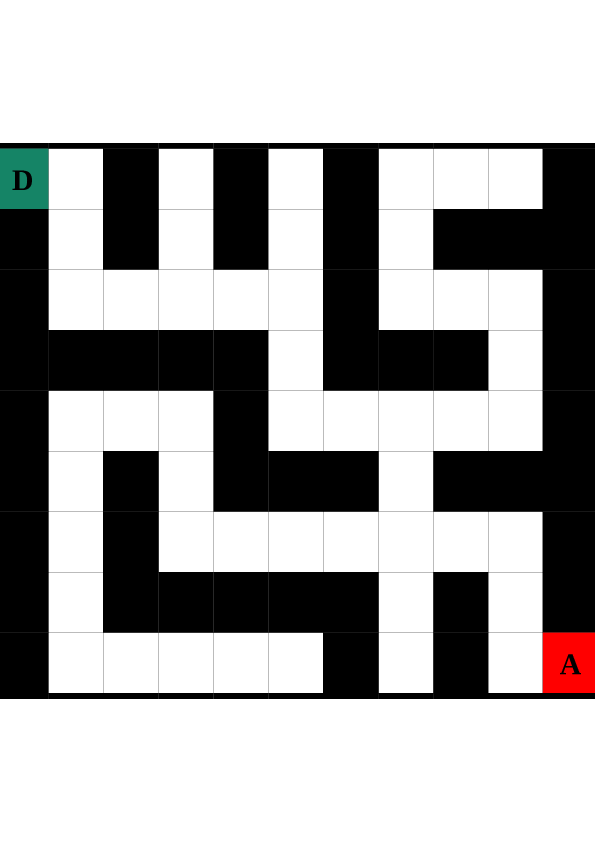
\includegraphics[width=\linewidth]{../diapos/page1.png}}    
  \end{minipage}
\end{frame} % Titre

\begin{frame}
  \frametitle{Table des matières}
  \tableofcontents
\end{frame} % toc

\section{Quel algorithme pour résoudre quel problème?}
\subsection{Choix du problème}
\begin{frame} 
  \frametitle{Un labyrinthe, plusieurs problèmes}
  \begin{itemize}
  \item<1-> Cherche-t-on un chemin quelconque?
    \begin{itemize}
    \item<2-> Oui, on ne traversera le labyrinthe qu'une seule fois.
    \item<2-> \textbf<3->{On veut le chemin le plus court}, pour peut-être le réutiliser.
    \end{itemize}
  \item<4-> Connait-on les coordonnées de la sortie dès le départ?
    \begin{itemize}
    \item<5-> \textbf<6->{Oui, et cette information pourra nous aider.}
    \item<5-> Non, le lieu de la sortie partie des inconnues.
    \end{itemize}
  \end{itemize}
\end{frame} % choix du problème

\subsection{Choix de l'Algorithme}
\begin{frame}
  \frametitle{Un problème, plusieurs solutions}
  \begin{itemize}
  \item<1-> Breadth-First Search
    \begin{itemize}
    \item garantit de trouver une solution si elle existe
    \item solution optimale si tous les pas sont égaux
    \end{itemize}
  \item<2-> Dijkstra
    \begin{itemize}
    \item choisit où explorer selon les distances déjà parcourues
    \item garantit de trouver le plus court chemin
    \end{itemize}    
  \item<3-> A*
    \begin{itemize}
    \item nécessite de connaître les coordonnées de la sortie
    \item choisit où explorer selon les distances déjà parcourues et la distance
      à la sortie
    \end{itemize}
  \end{itemize}
\end{frame}

\section{Algorithme A*}
\subsection{Pseudo-Code}
\begin{frame}
  \frametitle{Algorithme A*}
  \begin{block}{pseudo-code}
    Démarrer une file d'attente avec la cellule de départ $D$, une liste de
    prédécesseurs avec $\{D:Nil\}$ et une liste de coûts d'accès avec
    $\{D:0\}$.
    \medskip
    
    \onslide<2->{Tant que la file d'attente n'est pas vide,}
    \begin{itemize}
    \item<3-> extraire (pop) la cellule prioritaire $C$ de la file d'attente
    \item<4-> si $C$ est la cellule d'arrivée $A$, retourner le chemin qui y amène
          (via backtracking sur les prédecesseurs)
    \item<5-> sinon, pour chaque vosin $V$ de $C$ qui n'est pas déjà accessible
      à moindre co'ut
      \begin{itemize}
      \item<6-> mémoriser le prédecesseur de $V$ et le coût d'accès à $V$
      \item<7-> ajouter $V$ à la file d'attente
      \end{itemize}
    \end{itemize}    
  \end{block}
\end{frame}

\subsection{Heuristique et Priorité}
\begin{frame}
  \frametitle{Heuristique et Priorité}
  La priorité d'une cellule $C$ en attente est le coût estimé d'un chemin
  complet passant par cette cellule.
  \smallskip

  priorité = coût_réel ($D$ -> $C$) + coût_estimé ($C$ -> $S$)

  \medskip
  \onslide<2->{La distance restante depuis une cellule jusqu'à l'arrivée doit être estimée
  \textit{sans jamais surestimer}.}
  \begin{itemize}
  \item<3->{La \textbf{distance de Manhattan} $|\Delta x| + |\Delta y|$
    est un bon estimateur si les mouvements permis sont horizontaux et verticaux.}
  \par
  \item<4>{Une \textbf{heuristique nulle} ramène A* à l'algorithme de Dijkstra
      (ou Breadth-First Search sur grille carrée).}
  \end{itemize}
\end{frame}

\subsection{Structure de données ``Priority Queue''}
\begin{frame}
  \frametitle{File d'attente: ``Priority Queue''}
  \begin{itemize}
  \item Structure permettant insertion avec priorité et ``pop'' rapide de
    l'élément prioritaire
  \item Implémentation en Python en tant que \textbf{binary heap} avec le module \textit{heapq}
  \item Dans cette implémentation, vérifier si vide en $O(1)$, insertion et
    ``pop'' en $O\left(\log(n)\right)$ où $n$ est le nombre d'objets en attente\footnote{cf. https://www.cs.princeton.edu/~wayne/kleinberg-tardos/pdf/BinomialHeaps.pdf}
  % \item Un élément est un tuple (heuristique, numéro, contenu), ainsi en cas
  %   d'heuristique égale, le numéro le plus bas (insertion plus ancienne) donne
  %   la priorité
  \end{itemize}
\end{frame}
\begin{frame}
  \frametitle{Priority Queue pour A*}
  \begin{itemize}
  \item<1-> La priorité d'un noeud est le \textbf{coût heuristique} pour aller de
    l'entrée à la sortie en passant par ce noeud.
  \item<2-> Un élément de la queue a comme attributs l'identité du noeud, le
    \textbf{coût réel} pour y accéder et son prédecesseur
  \item<3-> La queue est initialisée avec le noeud de départ et un coût nul.
  \end{itemize}
\end{frame}

\subsection{Idée de preuve}
\begin{frame}
  \frametitle{Idée de preuve}
  Si l'heuristique sous-estime le coût du chemin futur, alors on arrive à un
  noeud toujours par un chemin de distance minimale d'abord.

  [à expliquer]
\end{frame}

\subsection{Exemple de résolution}
\begin{frame}
  \frametitle{Exemple de résolution}
  \begin{minipage}{.4\textwidth}    
    \only<1>{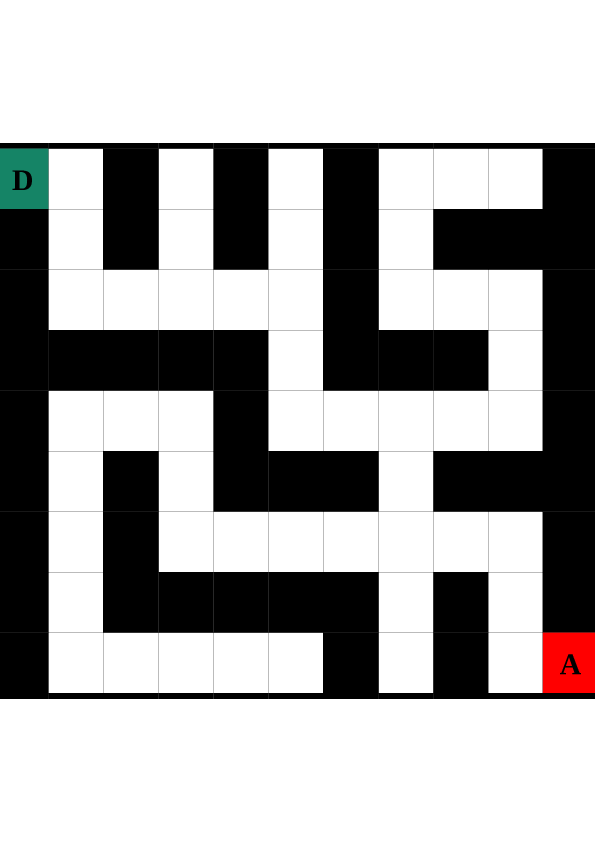
\includegraphics[width=\linewidth]{../diapos/page1.png}}
    \only<2>{\includegraphics[width=\linewidth]{../diapos/page3.png}}
    \only<3>{\includegraphics[width=\linewidth]{../diapos/page2.png}}
    \setcounter{pngnumber}{7}
    \forloop{onlynumber}{4}{\value{onlynumber} < 46}{
      % \only<\arabic{onlynumber}>{only \theonlynumber, png \thepngnumber}\par
      \only<\arabic{onlynumber}>{\includegraphics[width=\linewidth]{../diapos/page\arabic{pngnumber}.png}}
      \stepcounter{pngnumber}
    }
  \end{minipage}
  \quad
  \begin{minipage}{.55\textwidth}
    \only<1>{\textbf{Objectif}\par
      Trouver le chemin le plus court entre le \textbf{D}épart
      et l'\textbf{A}rrivée}
    \only<2>{Chaque noeud est à une distance réelle de l'arrivée, mais ces
      distances ne sont pas encore connues.}
    \only<3>{Le départ est mis en file d'attente, avec une priorité 0.}
    \only<4>{Le seul voisin est évalué:
      \begin{itemize}
      \item coût réel pour y accéder: \textcolor{green}1
      \item coût heuristique pour la suite: \textcolor{red}{17}
      \item coût heuristique total (priorité): 18
      \end{itemize}
    }
    \only<5-26>{
      Légende:
      \begin{itemize}
      \item\textcolor{green}{coût réel jusqu'ici}
      \item\textcolor{red}{coût heuristique pour la suite}
      \item {coût heuristique total}
      \end{itemize}
      \medskip
      L'algorithme poursuit son chemin.}
    \onslide<15,19,20>{\par Parfois deux choix ont la même priorité.}
    \only<27->{Un chemin vers la sortie a été trouvé!}
    \onslide<28->{Backtracking pour reconstituer le chemin}
  \end{minipage}
\end{frame}

\section{Complexité}
\begin{frame}
  \frametitle{Complexité}
  Le pire des cas sera réalisé par un labyrinthe dont le meilleur chemin revient
  souvent en arrière (s'éloigne de l'arrivée). Dans ce cas, aucun gain n'est
  réalisé par rapport à l'algorithme de Dijsktra.
\end{frame}

\section{Tests avec Python}
\begin{frame}
  \frametitle{Tests avec Python}
  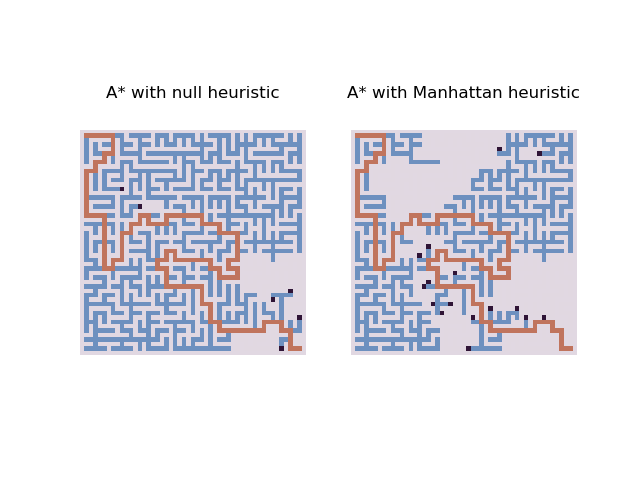
\includegraphics[width=.9\linewidth]{manhattan_vs_null.png}
\end{frame}

\section{Conclusion}
\begin{frame}
  \frametitle{Conclusion}
  \begin{itemize}
  \item \ldots
  \item Robot-Aspirateur
  \end{itemize}
\end{frame}

\end{document}